\chapter{Test Bed}
\label{chp:testbed}

We setup our testbed in a 8m X 6m office space. Sensors are mounted on the ceiling which is at a height of 3m. The sensors are  placed 2.5m apart in the horizontal direction and 2.2m apart in the vertical direction. We use  PIR sensor, EKMB1101112 from Panasonic. 
The output of the sensor is binary, with 1 indicating occupancy and 0 if the region is unoccupied.  We use eZ430-RF2500 toolkit which consists of MSP430 micro-controller  and CC2500 multi-channel
RF transceiver which is designed for low power wireless applications. The testbed uses simpliciTI a TI proprietary  low-power RF network protocol. To avoid collision we employ CSMA/CA. We place 8 sensors in the room as shown in the figure \ref{fig:roomLayout}. All the 8 nodes communicate directly to a centrally located access point which is connected to a laptop, which stores the data.
To decrease the packet loss we enable acknowledgment. An acknowledgment (ack) is sent from the AP if the packets are received. If no ack is received by a node, the node retransmits its data a maximum of 6 times until an ack is  received from the AP. If no ack is received even after retransmission the packet is dropped and the node continues carrying on its function. In the figure \ref{fig:packetLoss} we can see that the there was a decrease in the packet loss per node. The maximum packet loss before enabling acknowledgment was 23\%, after acknowledgment was enabled maximum packet loss for a node was 2\%.

\begin{figure}
\centering
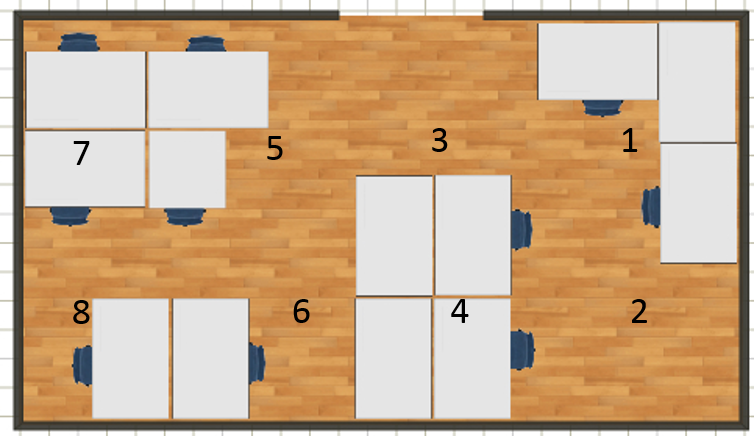
\includegraphics[scale=0.5]{./pics/roomLayout.png}
\caption{Room layout of the testbed.}
\label{fig:roomLayout}
\end{figure}

 We sample the PIR sensor every 100ms.All the nodes have a local clock running on them. With 1 clock tick corresponding to 1ms. All the local clocks are synchronized to one global clock. Since the data is binary we combine 32 samples and transmit the packet every 3.2s. 
Data packet is an array of 8 bit. The packet structure is as shown in the figure \ref{fig:packetStructure}\\


\begin{figure}
    \centering
    \begin{subfigure}[b]{1\textwidth}
        \centering
        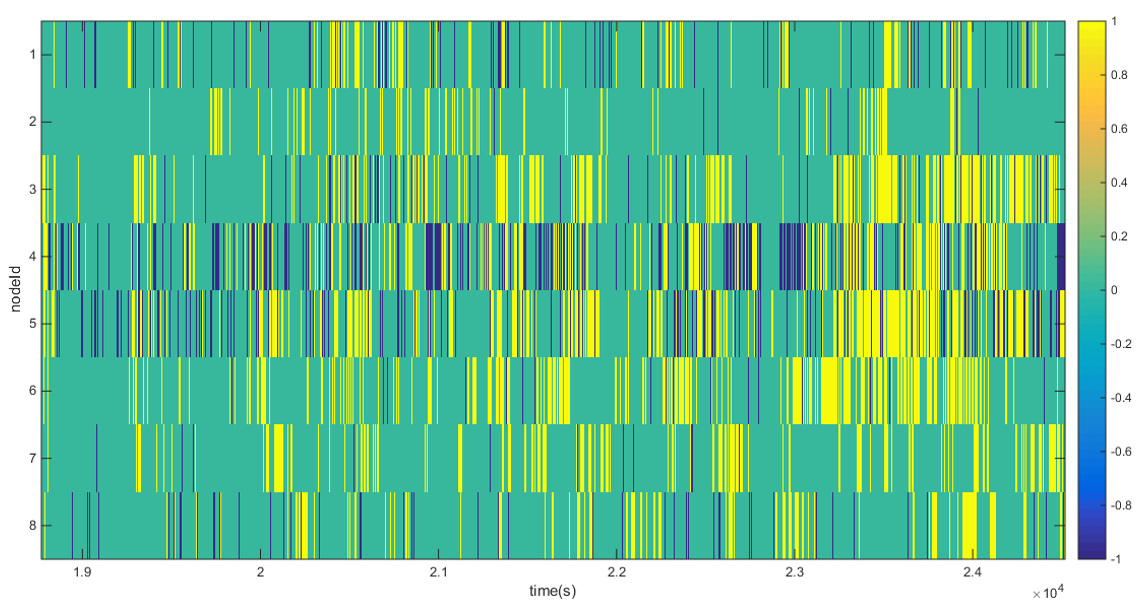
\includegraphics[width=8cm,height=4cm]{./pics/packetLoss.png}
      \caption{Data before ack was enabled}
       % \label{fig:y equals x}
    \end{subfigure}
    \hfill
    \begin{subfigure}[b]{1\textwidth}
        \centering
        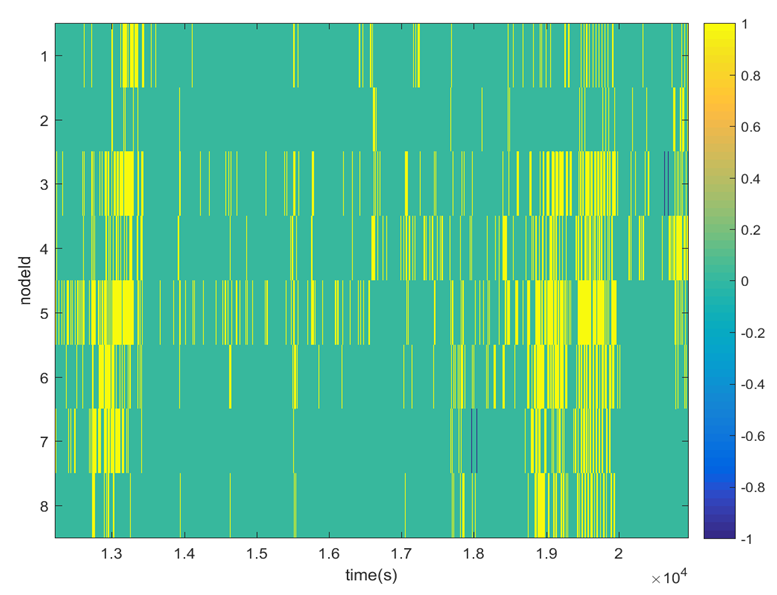
\includegraphics[width=8.5cm,height=4cm]{./pics/dataAfterAck.png}
        \caption{Data after ack was enabled}
        %\label{fig:three sin x}
    \end{subfigure}
\caption{Data from the test bed. - 1 indicates the lost data , 1 indicates occupancy, 0 indicates unoccupied space}
\label{fig:packetLoss}
\end{figure}

\begin{figure}
 \bytefieldsetup{bitheight=3em}
\begin{bytefield}[bitwidth=2.5em]{14}
\bitheader{0-13} \\
\bitbox{1}{\tiny Mac id} & \bitbox{1}{\tiny packet number} &
\bitbox{4}{start time}
& \bitbox{4}{end time} & \bitbox{4}{data}
\end{bytefield}.
\caption{Packet Structure}
\label{fig:packetStructure}
\end{figure}
The transmitted packet is an array of 1 byte. Consisting of 14 bytes of payload. The payload structure is as shown in the figure \ref{fig:packetStructure}
\begin{itemize}
\item Mac Id - unique identifier for each node.
\item Packet number- Keeps track of the packets that are being transmitted from a  node. It helps to identify the lost packets as well as repeated packets.
\item Start time - The time stamp corresponding to the first PIR sample of the PIR sensor in the packet.
\item End time - The time stamp corresponding to the last sample of the PIR sensor in the packet.
\item Data - 32 samples of the PIR sensor.
\end{itemize}

Data was collected for a span of 2 months. During the course of the evaluation, the occupants were notified of data gathering, but were never instructed to behave in any particular way or was there any constrained applied on the activity or the number of people in the room. 

\begin{figure}
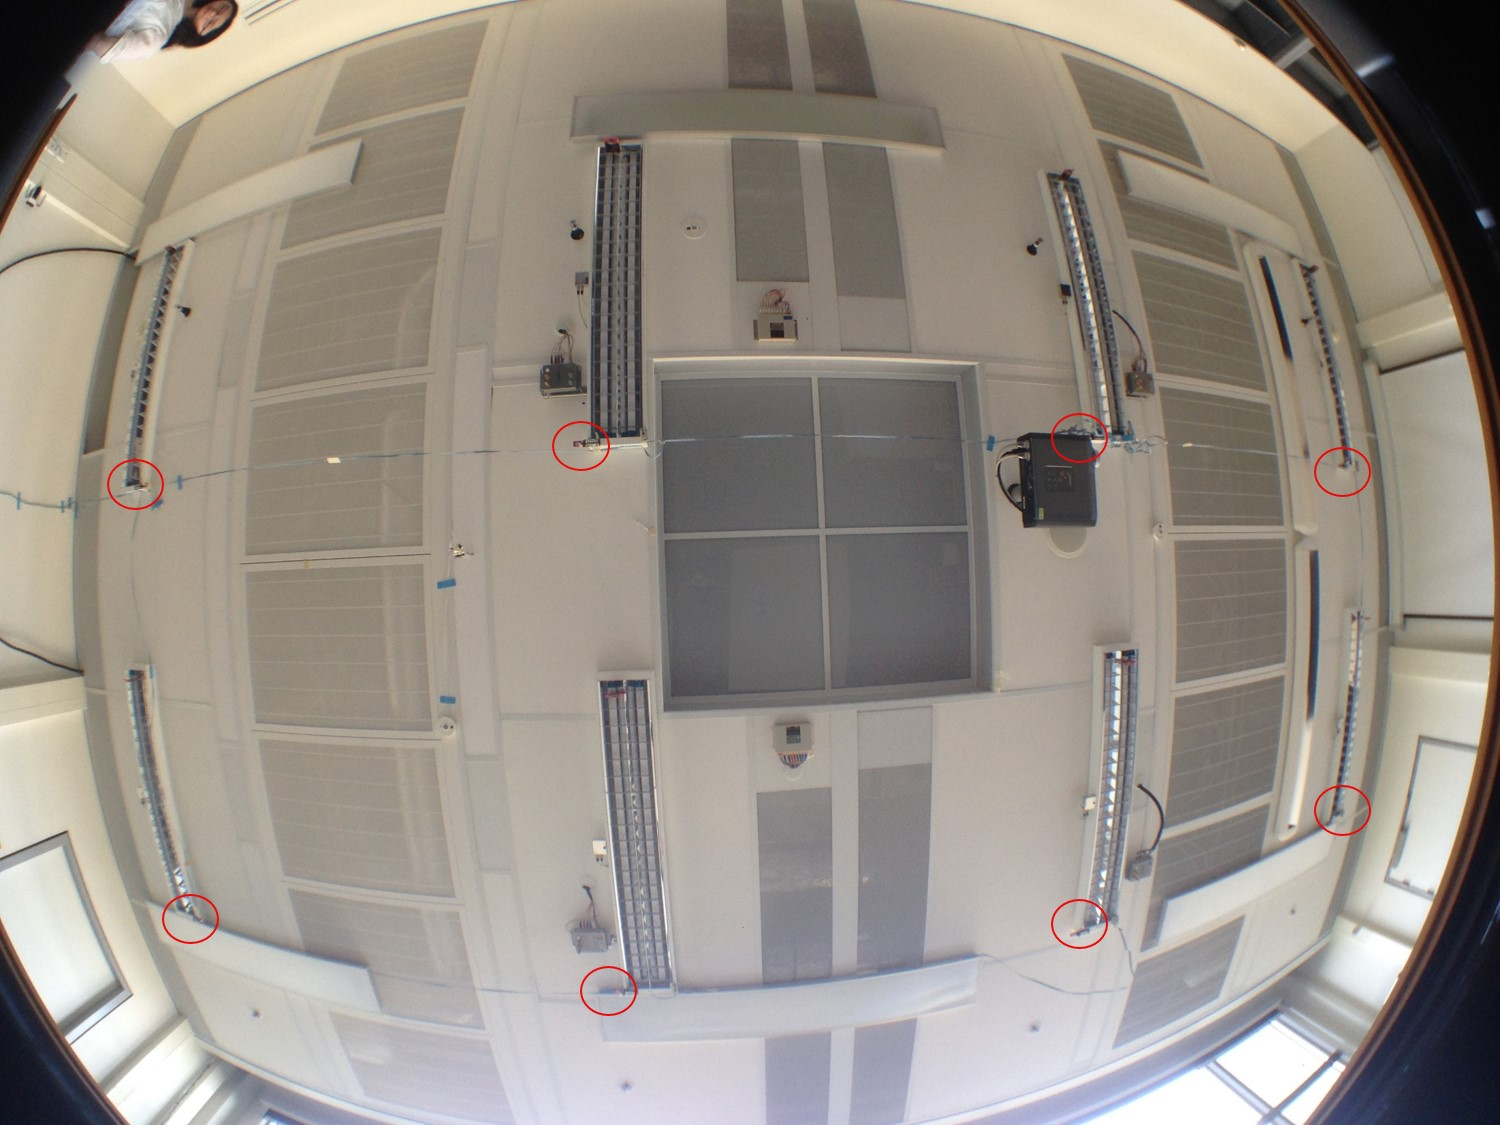
\includegraphics[scale=0.5]{./pics/lab_photo.jpg}
\caption{Photo of the lab setup with the sensors highlighted in red}
\end{figure}